\section{Software Interface}
\label{sec:software}

The primary design goals of the FlashBoost software are to manage NAND flash,
hiding its physical properties,
while offering easy-to-use interfaces 
between user-level applications and hardware accelerators in the storage device.

NAND flash has very different characteristics from traditional hard disk drives,
so a flash-aware management layer like a Flash Translation Layer (FTL)~\cite{}
is required to hide such differences from the rest of the system.
To this end, we employed a refactored I/O architecture
that offloads almost all of the FTL functions into a log-structured file system, called RFS~\cite{}.
Unlike conventional FTL designs where the flash characteristics are
hidden from the file system, RFS performs some functionality of an FTL,
including logical-to-physical address mapping and garbage collection.
This helps achieve achieving better garbage collection
efficiency at much lower memory requirement. For the sake of compatibility with
existing software, FlashBoost also offers a full-fledged page-level FTL for
end-users, which is implemented in the device driver, much like Fusion IO’s
driver implementation. It allows us to use well-known Linux file systems (e.g., ext2/4/3) 
as well as database systems (directly running on top of a block device) with FlashBoost.

%The most important feature of the FlashBoost software stack is that it provides
%easy-to-use software interfaces for application-specific hardware accelerators, 
%allowing developers to easily make use of fast near-data processing 
%without any efforts to write their own custom interfaces manually. 
The FlashBoost software allows developers to easily make use of fast near-data processing 
without any efforts to write their own custom interfaces manually. 
Figure~\ref{fig:filesystem} shows how user-level applications access hardware accelerators.
In the FlashBoost software stack, user-level
applications can provide the near-data processing engines with the physical
locations of data in the flash. 
Such physical locations can be easily obtained from the file
system (i.e., RFS) or the device driver, because they maintain the mapping
information between user files and flash storage (see (1) in Figure~\ref{fig:filesystem}). 
User-level applications then send queries together with physical addresses (2).
The in-store processor reads data from NAND flash directly and performs its analytic jobs (3).
Once the in-storage processor
finishes processing on the provided data, it will write the results to a host
memory region and notify the user application (4).

Since data analytics are done by well-optimized application-specific hardware and 
actual data transfers between the host and the storage device are avoided,
it greatly improves the performance of data analytics.
It is worth noting that, in FlashBoost,
all the user requests, including both user queries and data, are sent to the hardware directly, 
bypassing almost all OS kernel, except for essential driver modules. 
This helps us to avoid deep OS kernel stacks that often cause long I/O latencies. 
 
It is also very common that multiple
user-applications compete for the limited and precious hardware acceleration
units. For efficient sharing of hardware resources, FlashBoost runs a scheduling
daemon that assigns available hardware-acceleration units to competing
user-applications. In our implementation, a simple FIFO-based policy is used for
request scheduling.

\begin{figure}[h]
	\begin{center}
	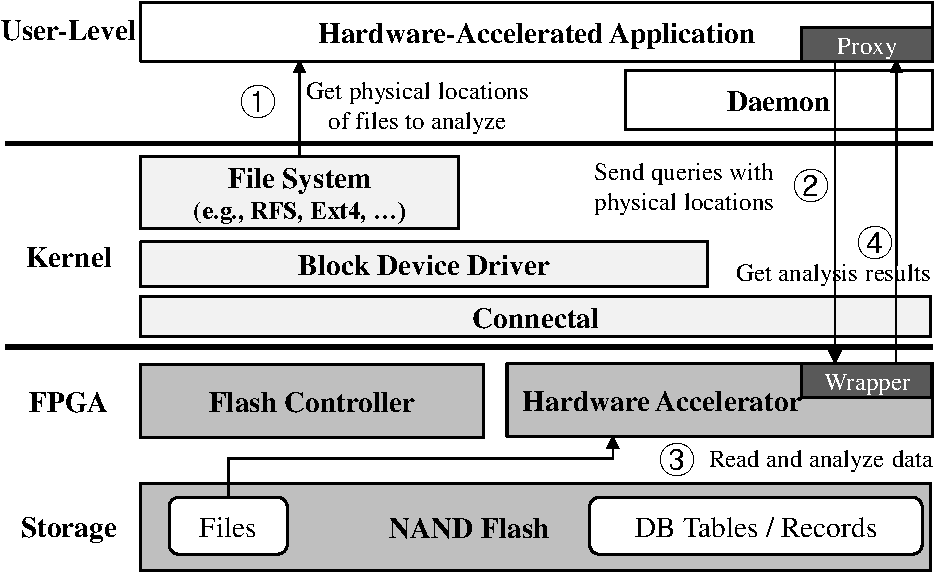
\includegraphics[width=0.4\paperwidth]{figures/software.pdf}
	\caption{File System Interface}
	\label{fig:filesystem}
	\end{center}
\end{figure}
